\section{Analyse bivariée}

\begin{frame}
	\begin{itemize}
	\item Même Données entrantes
	
	\begin{itemize}
		\item 814 rapport, avec les précurseurs de risque. 
		\item On a aussi obtenu les valeurs de l'evenement en pire cas, avec un deplacement spatio-temporel.
	\end{itemize}	
	
	\item On recalcule la valeur des $RR_p$ en fonction des pire cas.
	\item On recalcule la valeur des $R_{rapport_t}$ en fonction des pire cas.
	\item On fait le graphique des valeur des risque en pire cas en fonction des risques reels.

	\end{itemize}

\end{frame}

\begin{frame}
	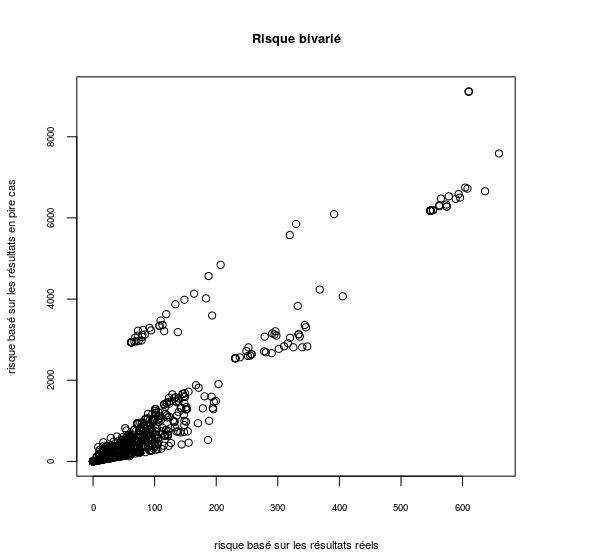
\includegraphics[width=220px, height=220px]{risque_bivarie}	
\end{frame}


\begin{frame}
	L'auteur suggère aussi une correspondance entre une valeur de risque 
	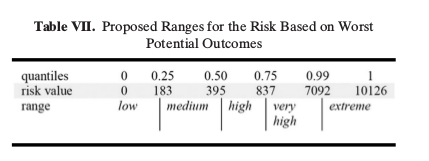
\includegraphics[width=\paperwidth]{range_propose_pire}	
\end{frame}


\begin{frame}
	Si on enleve l'effet de la fonction de répartition dans les données et qu'on ordonne chaque point selon son rang dans le jeu de donnes on obtient
	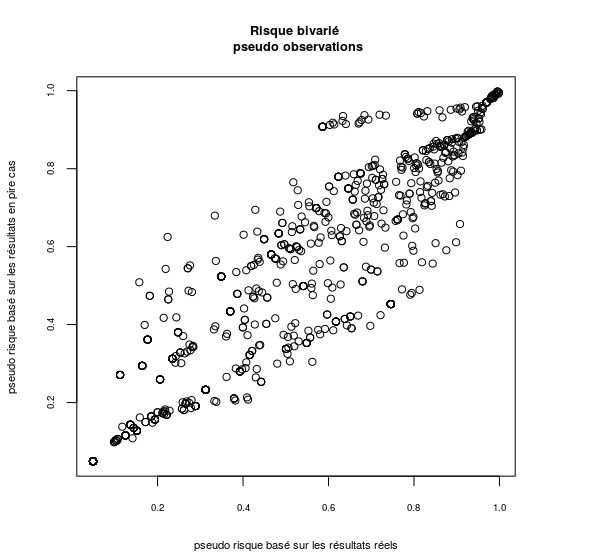
\includegraphics[width=220px, height=220px]{pseudo_risque_bivarie}	
	
\end{frame}


\begin{frame}
	Théorie des copules
	\begin{itemize}
		\item Utilisation d'une copule non paramétrique
		\item On appliquer une KDE sur deux dimensions (les rangs des observations)
		\item On appliquer une autre transformation 
		\item Technique proposée par \cite{charpentier}
		
	\end{itemize}
	Voir exemple en R (plotly)
	
\end{frame}



\begin{frame}
	Topographie de la copule
	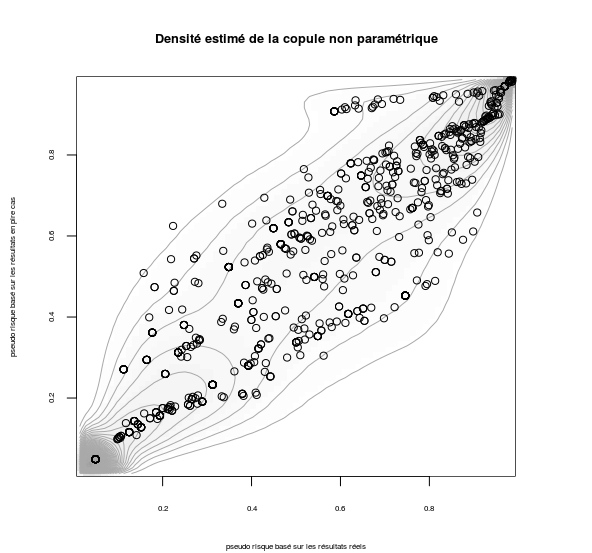
\includegraphics[width=220px, height=220px]{topographie_copule}	
	
\end{frame}


\begin{frame}
	Evaluation de l'escalation possible des risques
	\begin{itemize}
	\item On recréer des simulations grâce à la méthode bootstrap 
	\item On refait un graphiquefait une analyse bivariée des risques
	\end{itemize}
\end{frame}
	

\begin{frame}
	Evaluation de l'escalation possible des risques
	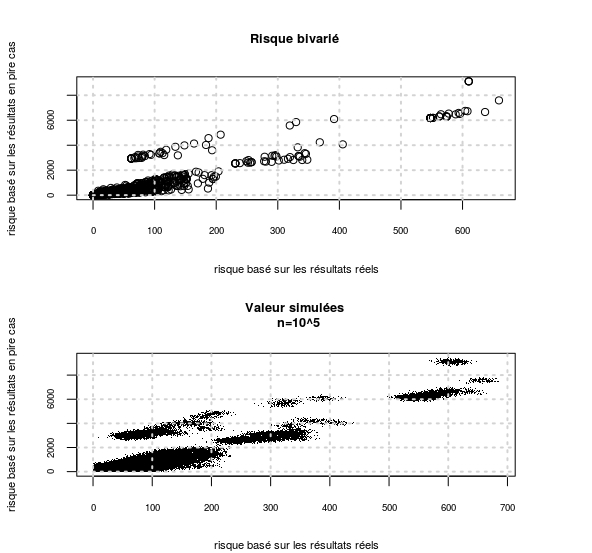
\includegraphics[width=220px, height=220px]{real_vs_simul}	
\end{frame}



\begin{frame}
	Calcul de l'escalation possible
	
	\begin{itemize}
		\item Calculer une valeur pour un risque $x_0$ telle que\\
		$x_0 = \sum_{p=1}^{P} RR_p * \delta_{rp}$\\
		avec $\delta_{rp}$ = 1 si le précurseur est présent dans le rapport et 0 autrement.
		\item On évalue $y_0 = P[R_{pire-cas}|x_0 - c < R_{réel}< x_0 + c ]$, \\
		avec $c=5$ choisi de façon arbitraire
		\item Pour calculer $y_0$, on sélection dans les données simulées les valeurs de risque en pire cas pour lesquels le risque en réel est $x_0 \pm c$.
	\end{itemize}
	
\end{frame}



\begin{frame}
	Évaluation du potentiel d'escalation de deux situations
	
	\begin{itemize}
	
	\item \textit{The employee was welding overhead and the wind shifted, resulting in discomfort in eye.}
		\begin{itemize}
			\item welding, working overhead, wind
			\item $x_0 = 10+1+6 = 17$
			\item 80e percentile de $y_0 = 290$
			
		\end{itemize}	
	\end{itemize}
	
	
	\begin{itemize}
	\item \textit{Worker is unloading a ladder from pickup with bad posture.}\\
	\begin{itemize}
		\item Ladder, Manual handling, Light vehicule, Improper body positionning
			\item $x_0 = 15 + 49 + 7 + 3 = 74  $
			\item quantiles de $y_0 = 897$
		\end{itemize}	
	\end{itemize}

	
\end{frame}

